\documentclass[11pt,paper=a4,answers]{exam}
\usepackage{graphicx,lastpage}
\usepackage{upgreek}
\usepackage{censor}
\usepackage{gensymb}
\usepackage{amsmath}
\usepackage{multicol}
\usepackage{enumitem}
\usepackage{tasks}
\usepackage{adjustbox}
\usepackage{xcolor}
\usepackage{tfrupee}
\setlength{\voffset}{0.25in}
\usepackage{tabularx}
\newcolumntype{Y}{>{\centering\arraybackslash}X}
%==============================================================
% Customise Non-Essential Packages Below
% =============================================================
\usepackage[most]{tcolorbox}
\usepackage{eso-pic}
\usepackage{tikz}
\AddToShipoutPictureBG{%
\begin{tikzpicture}[remember picture,overlay]
\foreach \x in {-8,-4,0,4,8,12,16,20}
\foreach \y in {-8,-4,0,4,8,12,16,20} {
\node[opacity=0.05,rotate=45,anchor=center] at ([xshift=\x cm,yshift=\y cm]current page.center) {%
\begin{minipage}{2cm}
\centering
\includegraphics[width=2cm]{images/logo_black.png}\\
\small preppeo.com
\end{minipage}%
};
}
\end{tikzpicture}%
}
\printanswers

%==============================================================
% Customise Non-Essential Packages Above
% =============================================================
\definecolor{svgray}{rgb}{0.90, 0.90, 0.90}
\graphicspath{{images/}}

\usepackage[normalem]{ulem}
\renewcommand\ULthickness{1pt}   %%---> For changing thickness of underline
\setlength\ULdepth{3.5ex}%\maxdimen ---> For changing depth of underline
\renewcommand{\baselinestretch}{1}
\chead{
\includegraphics[scale=0.1,height=2cm ]{logo.png}
}
\pagestyle{empty}

\pagestyle{headandfoot}
\headrule
\cfoot{W: https://preppeo.com; M: +91-8130711689}

\begin{document}
%==============================================================
% Customise Question paper details below this
% =============================================================
\begin{center}
    \centering
    \renewcommand{\arraystretch}{1.5}
    \begin{tabularx}{\textwidth}{YYY}
    & \normalsize\bf{{\Large{{Quant}}}} & \\
    By Preppeo & \normalsize\bf{{psda\_sat\_hard\_mcq\_003}} & SAT\\
    \normalsize{{\textbf{{Algebra}} }} & \normalsize{{\textbf{{ratio,probability, statistics }} }} & \normalsize{{\textbf{{Solving Linear Equations}} }} \\
    \end{tabularx}
\end{center}
\par\noindent\rule{\textwidth}{1pt}
% =============================================================
% Customise Question paper details above this
% =============================================================

\begin{questions}
\pointsinrightmargin
\pointsdroppedatright
\marksnotpoints
\pointpoints{mark}{marks}
\pointformat{\boldmath\themarginpoints}
\bracketedpoints

% =============================================================
% Question Begin
% =============================================================

\section*{SAT Advanced Math - Practice Set 14 (Easy with TikZ)}

% Q1: Based on x^2 - 5 Difference of Squares logic
\question
Which of the following expressions is equivalent to $x^2 - 7$?
\begin{tasks}(2)
    \task $(x + \sqrt{7})^2$
    \task $(x - \sqrt{7})^2$
    \task $(x + \sqrt{7})(x - \sqrt{7})$
    \task $(x + 7)(x - 1)$
\end{tasks}

\begin{solution}
This follows the difference of squares pattern: $a^2 - b^2 = (a+b)(a-b)$.
\vspace{5pt}
\begin{center}
Here, $a = x$ and $b = \sqrt{7}$ because $(\sqrt{7})^2 = 7$.
\end{center}
\vspace{5pt}
Answer: \colorbox{yellow!100}{C}
\end{solution}

\vspace{1cm}
% Q2: Based on 8x^10 Factoring logic
\question
Which of the following expressions is equivalent to $6x^{12} - 6x^{11} + 42x$?
\begin{tasks}(2)
    \task $x(5x^{12} - 5x^{11} + 41x)$
    \task $6x(x^{11} - x^{10} + 7)$
    \task $6x(x^{12} - x^{11} + 7x)$
    \task $6(x^{12} - x^{11} + 7x)$
\end{tasks}

\begin{solution}
Factor out the Greatest Common Factor (GCF), which is $6x$.
\vspace{5pt}
\begin{center}
$6x^{12} / 6x = x^{11}$ \\
$-6x^{11} / 6x = -x^{10}$ \\
$42x / 6x = 7$
\end{center}
\vspace{5pt}
Answer: \colorbox{yellow!100}{B}
\end{solution}

\vspace{1cm}

% Q3: Based on ry^4 Factoring logic
\question
The expression $80y^6 - 48y^5$ is equivalent to $ry^5(10y - 6)$, where $r$ is a constant. What is the value of $r$?
\begin{tasks}(2)
    \task 4 \task 8 \task 10 \task 16
\end{tasks}

\begin{solution}
Distribute the $r$ to match the original expression:
\vspace{5pt}
\begin{center}
$r \cdot 10 = 80 \implies r = 8$ \\
Check second term: $8 \cdot (-6) = -48$ (Matches).
\end{center}
\vspace{5pt}
Answer: \colorbox{yellow!100}{B}
\end{solution}

\vspace{1cm}

% Q4: Based on (1.5x - 2.4)^2 Decimal logic
\question
Which of the following is an equivalent form of $(2x - 1.5)^2 - (3x^2 - 4.5)$?
\begin{tasks}(2)
    \task $x^2 + 6.75$
    \task $x^2 - 6x + 6.75$
    \task $x^2 - 6x + 2.25$
    \task $-x^2 - 6x + 2.25$
\end{tasks}

\begin{solution}
Expand $(2x - 1.5)^2$: $4x^2 - 6x + 2.25$. \\
Subtract $(3x^2 - 4.5)$:
\vspace{5pt}
\begin{center}
$(4x^2 - 3x^2) - 6x + (2.25 + 4.5)$ \\
$x^2 - 6x + 6.75$
\end{center}
\vspace{5pt}
Answer: \colorbox{yellow!100}{B}
\end{solution}

\vspace{1cm}
% Q5: Ball Launch Interpretation - TIKZ ADDED
\question
The graph below shows the height $h$, in meters, of a ball $t$ seconds after it was launched from a platform.
\begin{center}
\begin{tikzpicture}[scale=0.8]
    \draw[step=1cm,gray!20,very thin] (0,0) grid (4,6);
    \draw[thick,->] (0,0) -- (4.5,0) node[right]{\tiny $t$ (sec)};
    \draw[thick,->] (0,0) -- (0,6.5) node[above]{\tiny $h$ (m)};
    \draw[ultra thick, blue, domain=0:2.2] plot (\x, {-2*(\x-0.8)^2 + 5.5});
    \filldraw (0.8, 5.5) circle (2.5pt) node[above]{\tiny $(0.8, 5.5)$};
    \foreach \x in {1,2,3,4} \node[below] at (\x,0) {\tiny \x};
    \foreach \y in {1,2,3,4,5,6} \node[left] at (0,\y) {\tiny \y};
\end{tikzpicture}
\end{center}
Which statement is the best interpretation of the marked point $(0.8, 5.5)$ in this context?
\begin{tasks}(1)
    \task 0.8 seconds after being launched, the ball's height is 5.5 meters.
    \task 5.5 seconds after being launched, the ball's height is 0.8 meters.
    \task The ball was launched from an initial height of 5.5 meters.
    \task The ball reached the ground after 5.5 seconds.
\end{tasks}

\begin{solution}
In the coordinate pair $(t, h)$, the $x$-value represents time and the $y$-value represents height.
\vspace{5pt}
Answer: \colorbox{yellow!100}{A}
\end{solution}

\vspace{1cm}

% Q6: Based on p(x) + 57 = x^2 (Minimum value)
\question
$p(x) + 32 = x^2$ \\
The equation above relates $x$ and $p(x)$. What is the minimum value of function $p$?
\begin{tasks}(2)
    \task -32 \task 0 \task 32 \task 1024
\end{tasks}

\begin{solution}
Isolate $p(x)$: $p(x) = x^2 - 32$.
\vspace{5pt}
\begin{center}
This is a parabola opening upward with vertex at $(0, -32)$.
\vspace{5pt}
The $y$-coordinate of the vertex is the minimum value.
\end{center}
\vspace{5pt}
Answer: \colorbox{yellow!100}{A}
\end{solution}

\vspace{1cm}
% Q7: Y-Intercept of Exponential Graph - TIKZ ADDED
\question
What is the $y$-intercept of the graph shown in the $xy$-plane below?
\begin{center}
\begin{tikzpicture}[scale=0.6]
    \draw[step=1cm,gray!20,very thin] (-4,-10) grid (4,2);
    \draw[thick,->] (-4,0) -- (4.5,0) node[right]{\tiny $x$};
    \draw[thick,->] (0,-10) -- (0,2.5) node[above]{\tiny $y$};
    \draw[ultra thick, red, domain=-2.1:4] plot (\x, {-0.5*3^(-\x) - 4.5});
    \filldraw[black] (0, -5) circle (3pt) node[right]{\tiny ?};
\end{tikzpicture}
\end{center}
\begin{tasks}(2)
    \task $(0, -4)$ \task $(0, -5)$ \task $(-5, 0)$ \task $(0, 0)$
\end{tasks}

\begin{solution}
The $y$-intercept is the point where the graph crosses the $y$-axis (where $x=0$). By observing the grid, the curve passes through $-5$ on the vertical axis.
\vspace{5pt}
Answer: \colorbox{yellow!100}{B}
\end{solution}

% Q8: Water Level Parabola Table - TIKZ ADDED
\question
The graph below models the water level $y$, in feet, over a period of $x$ hours. 
\begin{center}
\begin{tikzpicture}[scale=0.5]
    \draw[step=1cm,gray!15,very thin] (0,-14) grid (10,2);
    \draw[thick,->] (0,0) -- (10.5,0) node[right]{\tiny $x$};
    \draw[thick,->] (0,-14) -- (0,2.5) node[above]{\tiny $y$};
    \draw[ultra thick, violet, domain=0:8.5] plot (\x, {0.75*(\x-4)^2 - 12});
    \filldraw[black] (4, -12) circle (4pt) node[below]{\tiny $(4, -12)$};
\end{tikzpicture}
\end{center}
Which table gives a set of values $(x, y)$ that are consistent with the model?
\begin{tasks}(2)
    \task \begin{tabular}{|c|c|} \hline $x$ & $y$ \\ \hline 0 & 0 \\ \hline 4 & -12 \\ \hline \end{tabular}
    \task \begin{tabular}{|c|c|} \hline $x$ & $y$ \\ \hline 4 & 0 \\ \hline -12 & 4 \\ \hline \end{tabular}
    \task \begin{tabular}{|c|c|} \hline $x$ & $y$ \\ \hline 0 & 4 \\ \hline 0 & -12 \\ \hline \end{tabular}
    \task \begin{tabular}{|c|c|} \hline $x$ & $y$ \\ \hline 4 & 12 \\ \hline 0 & 0 \\ \hline \end{tabular}
\end{tasks}

\begin{solution}
The graph shows a vertex at $(4, -12)$. Table A includes this point and correctly identifies that the water level is near 0 at $x=0$.
\vspace{5pt}
Answer: \colorbox{yellow!100}{A}
\end{solution}

\vspace{1cm}


\vspace{1cm}
% Q9: Based on 6x - 9y > 12 Inequality
\question
Which of the following inequalities is equivalent to $8x - 12y > 20$?
\begin{tasks}(2)
    \task $x - y > 2.5$
    \task $2x - 3y > 5$
    \task $4x - 3y > 10$
    \task $3y - 2x > 5$
\end{tasks}

\begin{solution}
Divide all terms by the greatest common divisor, which is 4.
\vspace{5pt}
\begin{center}
$(8x/4) - (12y/4) > (20/4) \implies 2x - 3y > 5$.
\end{center}
\vspace{5pt}
Answer: \colorbox{yellow!100}{B}
\end{solution}

\vspace{1cm}

% Q10: Based on Linear-Quadratic System y = x + 1
\question
$y = x + 2$ \\
$y = x^2 + 2x$ \\
If $(x, y)$ is a solution to the system, which of the following could be the value of $x$?
\begin{tasks}(2)
    \task -2 \task -1 \task 0 \task 2
\end{tasks}

\begin{solution}
Set the equations equal: $x^2 + 2x = x + 2$.
\vspace{5pt}
\begin{center}
$x^2 + x - 2 = 0$ \\
$(x+2)(x-1) = 0$ \\
$x = -2$ or $x = 1$.
\end{center}
\vspace{5pt}
Answer: \colorbox{yellow!100}{A}
\end{solution}

\vspace{1cm}

% Q11: Difference of Squares (Simple)
\question
Which of the following is equivalent to $x^2 - 100$?
\begin{tasks}(2)
    \task $(x-10)^2$ \task $(x+50)(x-50)$ \task $(x+10)(x-10)$ \task $x(x-100)$
\end{tasks}

\begin{solution}
$100 = 10^2$. Pattern: $(x+10)(x-10)$.
\vspace{5pt}
Answer: \colorbox{yellow!100}{C}
\end{solution}

\vspace{1cm}

% Q12: Factoring with Negative Coefficients
\question
Which of the following is equivalent to $-3x^2 + 12x$?
\begin{tasks}(2)
    \task $-3x(x + 4)$ \task $-3x(x - 4)$ \task $3x(x + 4)$ \task $x(-3x - 12)$
\end{tasks}

\begin{solution}
Factor out $-3x$. Note that $12x / (-3x) = -4$.
\vspace{5pt}
Answer: \colorbox{yellow!100}{B}
\end{solution}

\vspace{1cm}

% Q13: Interpreting the Vertex in Context
\question
A quadratic function models the profit $P$ of a company $x$ years after 2010. If the vertex of the profit graph is $(5, 200)$, what does the 200 represent?
\begin{tasks}(1)
    \task The maximum profit was 200 thousand dollars.
    \task The profit was 0 in the year 200.
    \task The initial profit in 2010 was 200 thousand dollars.
    \task The company made profit for 200 years.
\end{tasks}

\begin{solution}
The $y$-value of the vertex in a profit model represents the maximum or minimum profit.
\vspace{5pt}
Answer: \colorbox{yellow!100}{A}
\end{solution}

\vspace{1cm}

% Q14: Distributing Negative Signs
\question
Which expression is equivalent to $-(x^2 - 4x) + (2x^2 - 5)$?
\begin{tasks}(2)
    \task $x^2 - 4x - 5$ \task $x^2 + 4x - 5$ \task $3x^2 + 4x - 5$ \task $x^2 + 4x + 5$
\end{tasks}

\begin{solution}
Distribute the negative: $-x^2 + 4x + 2x^2 - 5$. \\
Combine like terms: $x^2 + 4x - 5$.
\vspace{5pt}
Answer: \colorbox{yellow!100}{B}
\end{solution}

\vspace{1cm}

% Q15: Zeros of a Function - TIKZ ADDED
\question
If $f(x) = (x - 2)(x + 4)$, which of the following graphs could represent $y = f(x)$?
\begin{center}
\begin{tikzpicture}[scale=0.5]
    \draw[thick,->] (-5,0) -- (5,0) node[right]{\tiny $x$};
    \draw[thick,->] (0,-10) -- (0,5) node[above]{\tiny $y$};
    \draw[ultra thick, orange, domain=-4.5:2.5] plot (\x, {(\x-2)*(\x+4)});
    \node[below] at (2,0) {\tiny $2$};
    \node[below] at (-4,0) {\tiny $-4$};
\end{tikzpicture}
\end{center}
\begin{tasks}(2)
    \task $(2, 0)$ and $(-4, 0)$
    \task $(-2, 0)$ and $(4, 0)$
    \task $(0, 2)$ and $(0, -4)$
    \task $(2, 0)$ and $(4, 0)$
\end{tasks}

\begin{solution}
To find the $x$-intercepts (zeros), set each factor to zero:
\vspace{5pt}
\begin{center}
$x - 2 = 0 \implies x = 2$ \\
$x + 4 = 0 \implies x = -4$
\end{center}
\vspace{5pt}
The graph should cross the $x$-axis at $(2, 0)$ and $(-4, 0)$.
\vspace{5pt}
Answer: \colorbox{yellow!100}{A}
\end{solution}

% =============================================================
% Question End
% =============================================================

\end{questions}
\begin{center}
\rule{.5\textwidth}{1pt}
\end{center}
\end{document}
